\chapter{Results and Discussion}
\section{Population Behavior}

As we are trying to improve the model by making it more realistic, first, we included the stochasticity with probability distributions. Now I consider the fact that population is heterogeneous and has mixing nature. In dynamic models where mathematical tools of differential equations are applied, it is assumed that all individuals are the same and are continuously and uniformly mixed with each other in the modeled area. People have relationships and contact with other people like them in the same level and way. In fact, most populations have highly complex structure, in accordance with social stratification, a variety of geographical conditions and complex temporal and spatially simple movement patterns. In addition, classical dynamic models are fully deterministic and are only suitable for the evaluation of the behavior of very large populations. The nature of the epidemic processes is probabilistic; if ignoring the random factors and accidental incidences, it is possible get rough or incorrect simulation results.

In recent years, the largest contribution to the modeling the spread of diseases was made by so-called "population" (Population-based) models which were developed by I. M. Longini [9]. This is a discrete-event model, which reflects the trivial structure of the society: individuals are classified by their ages; in this case, the spread of the disease between people can only happen in a single contact group (different for each age category) [9]. Contact groups are determined by the characteristic structure of society, which will depend on the modeled area. For example, one contact group may include classmates, colleagues, family members, children, and so on.

Stages of the disease duration in a population based models usually correspond to the dynamic SEIR model. Time in population based models moves with fixed interval of discretization, usually 12 or 24 hours. At each step, we analyze the individuals’ visited places and by formula, taking into account various factors, calculate the probability of the event that individual is infected in the period of time.  Fixed interval of discretization and the calculation formula of contact rate are the main sources of errors in the population models. Moreover, the coefficients used in the formula require careful calibration which may be difficult to do if model contains administrative measures to fight the morbidity.

To cope with these complexities, I decided to build population based like model not with discrete event method as it’s usually made, but with system dynamics approach. So, I can divide the population into categories by ages and use system dynamics approach. This approach is based on the consideration of parallelism of multiple elements in the process, each of which is described by a set of deterministic and stochastic parameters that determine the characteristics of the "life cycle" of the element in the simulation. In such method, I assume that each person in a category represents the real world in the form of many separately-specified active subsystems. Each person communicates with others and in the operation can change their behavior and take into account the changes in external environment.

The number of people in each age group model is determined by demographic data in the modeled area. Age group characterizes important factors such as determining the probability of infection, the number of contacts with other people in a day and the possible visits of individuals (school, work, etc.). For example, a person from 7 to 18 years old can attend locations such as "home", "school" and "transport". If necessary, this list can be replenished. So, in average these children contact about 25 people a day as they go to school where there are around 20-25 people in a class.  So, people in each category has own parameters defined randomly. And each category is modeled separately with infection rates and recovery rates.

The number of people that are colonized with sensitive bacteria is always non-zero, i.e. such people are always present in the system. This happens because such individuals are constantly entering the hospital. The population that is free from bacteria colonization is also present, since this kind of people are constantly entering from outside, too, and infected people is cured. The number of people colonized with resistant bacteria may fall to zero or stay positive. If the transmission probabilities of resistant and sensitive stains are equal, then the latter case happens under the following condition:

\begin{equation}
R_0 > \tau_1/(\tau_1 - m \mu)
\end{equation}

Here, $R_0 = \beta/(\tau_2 + \mu + \gamma)$ is a special value that indicates the rate of resistant strain reproduction in an ideal case when all of the individuals entering the hospital are not colonized with bacteria at all.

We have executed the model simulation under several different parameter settings in order to understand the difference of population dynamics. In the first case, when the basic reproductive rate is large enough, the population infected by resistant bacteria strain has a sharp fall in the beginning, after which a gradual decrease follows, transforming into an almost constant value. The resistant bacteria population is sufficiently stable in this case.

\begin{figure}[H]
  \centering
  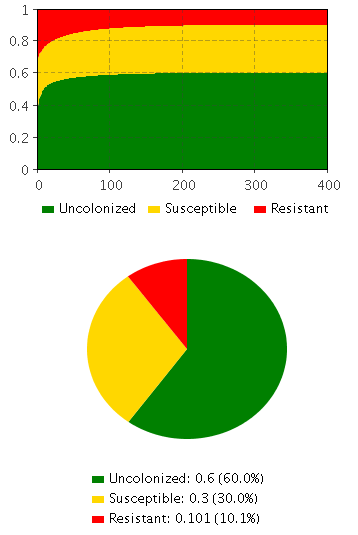
\includegraphics[height=0.7\textwidth]{img/screens/result/result1}
  \caption{The simulation dynamics of the model for the case when $R_0 > \tau_1/(\tau_1 - m \mu)$}
\end{figure}

When the basic reproductive rate is too small, the population infected by the resistant bacteria can not manage to survive under the treatment frequency of drug 2. This is why the population sharply decreases and almost disappeares from the hospital environment.

\begin{figure}[H]
  \centering
  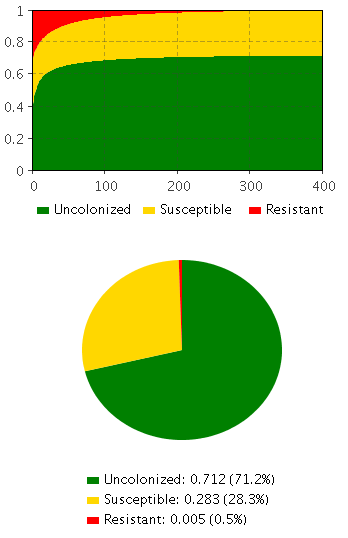
\includegraphics[height=0.7\textwidth]{img/screens/result/result2}
  \caption{Simulation results in case whent the basic reproductive rate is too small}
\end{figure}

There can be considered another extreme case, when the basic reproductive rate of the resistant strain is too high. In this case, the population infected by the resistant bacteria increases rapidly at the beginning, however becomes almost constant after some time. This phenomenon is probably happening due to presense of the second drug.

\begin{figure}[H]
  \centering
  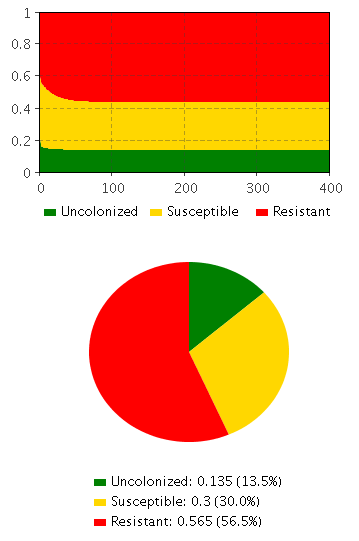
\includegraphics[height=0.7\textwidth]{img/screens/result/result3}
  \caption{Simulation with a very high basic reproductive rate}
\end{figure}
